\section{\AP{}Preliminaries}
\label{sec:prelim}

Before attacking the statement of our "Key Lemma" in \Cref{sec:maximal-under-approximations},
we first give a few elementary definitions on "C2RPQs" in this section.
%
% \paragraph*{Homomorphisms}
\AP
A homomorphism $\fun$ from a "C2RPQ" $\gamma(x_1, \dotsc, x_m)$ to a "C2RPQ" $\gamma'(y_1, \dotsc, y_m)$ is a mapping from $\vars(\gamma)$ to $\vars(\gamma')$ such that $\fun(x) \atom{L} \fun(y)$ is an "atom" of $\gamma'$ for every "atom" $x \atom{L} y$ of $\gamma$, and further $\fun(x_i)=y_i$ for every $i$.
Such a "homomorphism" $\fun$ is \AP""strong onto"" if for every "atom" $x' \atom{L} y'$ of $\gamma'$ there is an "atom" $x \atom{L} y$ of $\gamma$ such that $\fun(x)=x'$ and $\fun(y)=y'$.
An example of "homomorphism" is provided in \Cref{fig:basic-hom}.
We write $\gamma \homto \gamma'$ if there is a "homomorphism" from $\gamma$ to $\gamma'$, and $\gamma \surj \gamma'$ if there is a "strong onto homomorphism".
\todo{change this shit}
In the latter case, we say that $\gamma'$ is a \AP""homomorphic image"" of $\gamma$.
It is easy to see that if $\gamma \homto \gamma'$ then $\gamma' \contained \gamma$, and in the case where $\gamma,\gamma'$ are "CQs" this is an ``if and only if'' \cite[Lemma~13]{ChandraMerlin1977Implementation}.
% Similarly, for a tuple $\bar{v}$, we write $\gamma\homto (G, \bar{v})$ if there is a homomorphism $h$ from $\gamma$ to $G$  such that $h(\bar{x}) = \bar{v}$ and we write
% $h: \gamma\homto (G, \bar{v})$ to make such $h$ explicit.
%
% "Homomorphisms" and "strong onto homomorphisms" between CQs are essentially defined as before with the main difference that free variables must be mapped to free variables.
% That is, given two CQs $\gamma_1(\bar{x}_1)$, $\gamma_2(\bar{x}_2)$, we have $h: \gamma_1 \homto \gamma_2$ if $h:\gamma_1 \homto (G,\bar{x}_2)$, where $G$ is the graph database denoted by $\gamma_2$.
% A ""homomorphism"" $h$ from a "CQ" $\gamma(\bar{x})$ to a "graph database" $G=(V,E)$ is a mapping from $\vars(\gamma)$ to $V$ such that $h(x) \xrightarrow{a} h(y)$ belongs to $E$ for each "atom" $x \xrightarrow{a} y$ of $\gamma$. 
% Such a "homomorphism" $h$ is ""strong onto"" if for every edge $u \xrightarrow{a} v$ of $E$ there is an atom $x \xrightarrow{a} y$ of $\gamma$ such that $h(x)=u$ and $h(v)=v$.
% We write $\gamma \intro*\homto G$ if there is a "homomorphism" from $\gamma$ to $G$, and $\gamma \intro*\surj G$ if there is a "strong onto homomorphism".
% Similarly, for a tuple $\bar{v}$, we write $\gamma\homto (G, \bar{v})$ if there is a homomorphism $h$ from $\gamma$ to $G$  such that $h(\bar{x}) = \bar{v}$ and we write
% $h: \gamma\homto (G, \bar{v})$ to make such $h$ explicit.
% %
% "Homomorphisms" and "strong onto homomorphisms" between CQs are essentially defined as before with the main difference that free variables must be mapped to free variables.
% That is, given two CQs $\gamma_1(\bar{x}_1)$, $\gamma_2(\bar{x}_2)$, we have $h: \gamma_1 \homto \gamma_2$ if $h:\gamma_1 \homto (G,\bar{x}_2)$, where $G$ is the graph database denoted by $\gamma_2$.

\paragraph*{Some intuitions on maximal under-approximations}
Given a "conjunctive query" $\gamma$,
the union of all "conjunctive queries"
that are "contained" in $\gamma$ is "semantically equivalent" to the union
$\bigvee \{ \gamma' \mid \gamma \surj \gamma' \}$. Naturally, this statement borders on the trivial since $\gamma'$ belongs to this union. It becomes interesting when we add a restriction:
given a class $\class$ of "CQs" (to which $\gamma$ may not belong) closed under "subqueries", then $\Gamma' \defeq \bigvee \{ \gamma' \in \class \mid \gamma \surj \gamma' \}$ is the maximal under-approximations
of $\gamma$ by finite unions of "conjunctive queries" of $\class$, in the following sense:
% \begin{description}
% 	\item[class] $\Gamma'$ is a finite union of "CQs" of $\class$,
% 	\item[under-approximation] $\Gamma' \contained \gamma$, and
% 	\item[maximality] for any finite union $\Delta$ of "CQs" of $\class$, if $\Delta \contained \gamma$, then $\Delta \contained \Gamma'$.
% \end{description}
\begin{enumerate}[label=\roman*.]
	\item (finite) $\Gamma'$ is a finite union of "CQs" of $\class$,
	\item (under-approximation) $\Gamma' \contained \gamma$, and
	\item (maximality) for any finite union $\Delta$ of "CQs" of $\class$, if $\Delta \contained \gamma$, then $\Delta \contained \Gamma'$.
\end{enumerate}

\begin{proof}
Only the last point is non-trivial, and follows from the fact that if
$\Delta \contained \gamma$, then for each $\delta \in \Delta$, $\delta \contained \gamma$,
so there is a "homomorphism" $f\colon \gamma \to \delta$. The image $\delta'$
of $f$ is a "subquery" of $\delta$, and $\+C$ is closed under "subqueries",
so it belongs to $\+C$, and hence to $\Gamma'$. Since there is a trivial homomorphism
from $\delta'$ to $\delta$, we moreover have that $\delta \contained \delta'$.
Hence, for each "CQ" $\delta \in \Delta$, there is a CQ $\delta' \in \Gamma'$ such
that $\delta \contained \delta'$, and hence $\Delta \contained \Gamma'$.
\end{proof}

As a consequence, we deduce that for each $k \geq 1$,
the "maximal under-approximation" of a "CQ" by
a finite union of "CQs" of "tree-width" at most $k$ is computable, and hence
we can effectively decide if some "CQ" is "equivalent" to a query of "tree-width" at
most $k$ by testing the equivalence with this maximal under-approximation.
For more details on approximations of "CQs", see \cite{BarceloLibkinRomero2014Efficient}.
Note that interestingly, changing $\Gamma'$ from
$\bigvee \{ \gamma' \in \class \mid \gamma \surj \gamma' \}$
to $\bigvee \{ \gamma' \in \class \mid \gamma' \contained \gamma \}$
preserves both under-approximation and maximality, but $\Gamma'$ is now an infinite
union of "CQs" of $\+C$.

Unfortunately, these results cannot be straightforwardly extended to "conjunctive regular
path queries" since the previous proof implicitly relied on two points:
\begin{enumerate}
	\item the equivalence between the
	"containment" $\gamma' \contained \gamma$ and the existence of a "homomorphism"
	$\gamma \homto \gamma'$, and
	\item the possibility to restrict $\gamma'$ to its image $\gamma \homto \gamma'$ while 
	obtaining a semantically bigger query.
\end{enumerate}
These two crucial ingredients is what allows us to build a finite set $\Gamma'$ from $\gamma$.
For "CRPQs", the second point still holds, but not the first one.
For instance, the "CQ" $\gamma(x,y) = x \atom{a} z \atom{b} y$ is
contained in (in fact "equivalent" to) the "CRPQ" $\gamma'(x,y) = x \atom{ab} y$,
but there is no "homomorphism" from $\gamma'(x,y)$ to $\gamma(x,y)$.
Our main result shows that to find "maximal under-approximations" of "C2RPQs",
it suffices to take "homomorphic images" of so-called ``"refinements"'' of $\gamma$,
instead of "homomorphic images" of $\gamma$ itself. The next paragraphs are devoted to
introducing "refinements" and tools related to them.

\paragraph*{Equality Atoms}
\AP"C2RPQs" with ""equality atoms"" are queries of the form $\gamma(\bar{x}) = \delta \land I$, 
where $\delta$ is a "C2RPQ" (without equality atoms) and $I$ is a conjunction of "equality atoms" of the form $x=y$. 
Again, we denote by $\vars(\gamma)$ the set of variables appearing in the (equality and non-equality) atoms of $\gamma$. 
We define the binary relation $=_\gamma$ over $\vars(\gamma)$ to be the reflexive-symmetric-transitive closure of the binary relation $\{(x, y) \mid \text{$x=y$ is an "equality atom" in $\gamma$}\}$. 
In other words, we have $x=_\gamma y$ if the equality $x=y$ is forced by the "equality atoms" of $\gamma$. 
Note that every "C2RPQ" with "equality atoms" $\gamma(\bar{x}) = \delta \land I$ is equivalent to a "C2RPQ" without "equality atoms"  $\gamma^{\collapse}$, 
which is obtained from $\gamma$ by collapsing each equivalence class of the relation $=_\gamma$ into a single variable. 
This transformation gives us a \emph{canonical} renaming from $\vars(\gamma)$ to $\vars(\gamma^{\collapse})$. For instance, $\gamma(x,y) \defeq x \atom{K} y \land y \atom{L} z \land x = y$
collapses to $\gamma^{\collapse}(x,x) \defeq x \atom{K} x \land x \atom{L} z$.

\paragraph*{Refinements}
\AP An ""atom $m$-refinement"" of a "C2RPQ" "atom" $\gamma(x,y) = x \atom{L} y$ where $L$ is given by the NFA $\+A_L$ is any "C2RPQ" of the form 
\begin{equation}
    \AP\label{eq:refinement}
    \rho(x,y) = x \atom{L_1} t_1 \atom{L_2} \hdots \atom{L_{n-1}} t_{n-1} \atom{L_n} y
	%\tag{\adfdownhalfleafright}
\end{equation}
where $1 \leq n \leq m$, $t_1,\hdots,t_{n-1}$ are fresh (existentially quantified) variables,
and $L_1,\hdots,L_n$ are such that there exists a sequence $(q_0,\dotsc,q_n)$ of states of $\+A_L$
such that $q_0$ is initial, $q_n$ is final, and for each $i$, $L_i$ is either of the form
\begin{enumerate}[label=\roman*.]
	\item $\subaut{\+A_L}{q_i}{q_{i+1}}$,
	\item $\{a\}$ if the letter $a\in \A$ belongs to $\subaut{\+A_L}{q_i}{q_{i+1}}$, or 
	\item $\{a^{-}\}$ if $a^{-} \in \A^{-}$ belongs to $\subaut{\+A}{q_i}{q_{i+1}}$.
\end{enumerate}
Additionally, if $\epsilon \in L$, the "equality atom" ``$x = y$'' is also an \reintro{atom $m$-refinement}. Thus, an \reintro{atom $m$-refinement} can be either of the form \eqref{eq:refinement} or ``$x=y$''.
% Further, we assume that either $n=1$ or that no atom of $\rho$ is labelled with the language $\set{\epsilon}$.\sidediego{CHECK}
% \sideremi{Je suis pas sûr que $\{\varepsilon\}$ soit un problème : (c'est assez rare de produire
% un tel mot). En revanche, on devrait peut-être interdire $L_i = \varnothing$.
% En fait, pour pouvoir merger des variables, il faudrait autoriser $n = 0$, mais seulement
% lorsque $\varepsilon \in L$.}
% We call the atoms of the form (i) \AP""sublanguage atoms"" and atoms of the form (ii) or (iii) \AP""label atoms"".
By convention, $t \atom{a^{-}} t'$ is a shorthand for $t' \atom{a} t$. As a consequence,
the underlying graph of an "atom $m$-refinement" of the form \eqref{eq:refinement} is not necessarily a directed path.
By definition, note that
$L_1\cdots L_n \subseteq L$ and hence $\rho \contained \gamma$ for any "atom $m$-refinement" $\rho$ of $\gamma$.
An \AP""atom refinement"" is an "atom $m$-refinement" for some $m$.
An example is provided in \Cref{fig:basic-refinement}.

\begin{marginfigure}
	\centering
	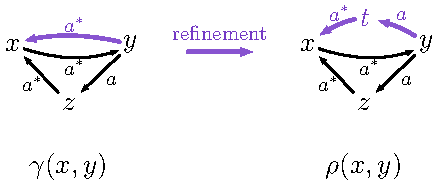
\includegraphics[width=\linewidth]{basic-refinement.pdf}
	\caption{\AP\label{fig:basic-refinement}A "refinement".}
\end{marginfigure}
	
\begin{marginfigure}
	\centering
	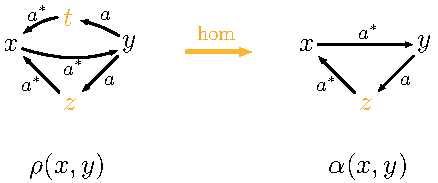
\includegraphics[width=\linewidth]{basic-hom.pdf}
	\caption{\AP\label{fig:basic-hom}A "strong onto homomorphism".}
\end{marginfigure}

\begin{definition}
    \AP\label{def:atom-contraction}
    \AP Given an "atom refinement" $\rho = x \atom{L_1} t_1 \atom{L_2} \hdots \atom{L_{n-1}} t_{n-1} \atom{L_n} y$ of $\gamma = x \atom{L} y$ as in \eqref{eq:refinement}, define
    a ""condensation"" of $\rho$ between $t_i$ and $t_j$, where $0 \leq i,j \leq n$ and $j > i+1$, as any "C2RPQ" of the form:
    \[
        \rho' = x \atom{L_1} t_1 \atom{L_2} \hdots \atom{L_i} \textcolor{cPurple}{t_i \atom{K} t_j} \atom{L_{j+1}} \hdots
        \atom{L_{n-1}} t_{n-1} \atom{L_n} y
    \]
    such that $\textcolor{cPurple}{K = \+A[q_i,q_j]}$.
	\begin{fact}
		\AP\label{fact:refinement-contained}
		Every "condensation" $\rho'$ of $\rho$ is a "refinement" of $\gamma$, and $\rho \contained \rho' \contained \gamma$.
	\end{fact}
    \AP Informally, we will abuse the notation and
    write $\intro*\contract{L_{i}\cdots L_{j}}$ to denote the language $K$---even if this language
    does not only depend on $L_{i}\cdots L_{j}$.
\end{definition}

\begin{example}
    \AP\label{ex:atom-refinement-twoway}
    Let $\gamma(x,y) = x \atom{(aa^-)^*} y$ be a "C2RPQ" "atom", where
    $(aa^-)^*$ is implicitly represented by its minimal automaton.
    Then $\rho(x,y)$ is a "refinement" of "refinement length" seven of $\gamma(x,y)$
    and $\rho'(x,y)$ is a "condensation" of $\rho(x,y)$, where:
    \begin{align*}
        \rho(x,y) & = x \atom{a} t_1 \atom{(a^-a)^*} t_2 \atom{(a^-a)^*} t_3
            \coatom{a} t_4 \atom{(aa^-)^*} t_5 \atom{(aa^-)^*a} t_6 \coatom{a} y, \\
        \rho'(x,y) & = x \atom{a} t_1 \atom{(a^-a)^*} t_2 \atom{(a^-a)^*} t_3
		\coatom{a} t_4 \atom{(aa^-)^*} y. 
    \end{align*}
    On the other hand, $\rho''(x,y) = x \atom{a} t_1 \coatom{a} y$ is not
    a "condensation" of $\rho(x,y)$.
\end{example}

Given a natural number $m$, an \AP""$m$-refinement"" of a "C2RPQ" $\gamma(\bar x) = \bigwedge_{i} x_i \atom{L_i} y_i$ is any query resulting from: 1) replacing every "atom" by one of its "$m$-refinements@@atom", and 2)
should some "$m$-refinements@@atom" have "equality atoms",
collapsing the variables.
\AP A ""refinement"" is an "$m$-refinement" for some $m$.
Note that any "atom $m$-refinements" is, by definition, also an
"atom $m'$-refinements" when $m \leq m'$: as a consequence, in the "refinement" of a "C2RPQ"
the "atom refinements" need not have the same length.
For instance, both $\rho(x,x) = x \atom{c} x$ and $\rho'(x,y) = x \atom{a} t_1 \atom{a} y \coatom{c} y$ are "refinements" of $\gamma(x,y) = x \atom{a^*} y \coatom{c} x$.

%%%%%%%%%%%%%%%%%%%%%
%     We will assume that a query "refinement" does not contain atoms with the language $\set{\epsilon}$; these are eliminated by identifying variables in a standard way. For example, if the result of replacing atoms by "atom refinements" yields $\gamma(x,z) = x \atom{\set{\epsilon}} y \land y \atom{\set{\epsilon}} z \land z \atom{a^*} x$ the associated "refinement" is then $\gamma(x,x) =  x \atom{a^*} x$.
% \sidediego{CHECK}
%%%%%%%%%%%%%%%%%%%%%
For a given "C2RPQ" $\gamma$, let $\AP\intro*\Refin[\leq m](\gamma)$ be the set of all "$m$-refinements" of $\gamma$, and $\reintro*\Refin(\gamma)$ be the set of all its "refinements".
Given a "refinement" $\rho(\bar x)$ of $\gamma(\bar x)$,
its ""refinement length"" is the least natural number
$m$ such that $\rho(\bar x) \in \Refin[\leq m](\gamma)$.
Note that if the automaton representing a language $L$ has more than one final state, for instance the minimal automaton for $L = a^+ + b^+$,
then $x \atom{L} y$ is not a "refinement" of itself.
However, it will always be "equivalent" to a union of refinements: in
this example, $x \atom{a^+ + b^+} y$ is "equivalent" to the union of
$x \atom{a^+} y$ and $x \atom{b^+} y$, which are both "refinements"
of the original "C2RPQ".

\paragraph*{Expansions}
%%%%%%%%%%%%%%%%%%%%%
% \sidediego{CHECK}
% Observe that a "C2RPQ" $\gamma$ whose every language is of the form $\set{z}$ for $z \in \Aext \dcup \set{\varepsilon}$ is equivalent to a "conjunctive query" $\tilde \gamma$. For example, $\gamma(x,y) = x \atom{\varepsilon} y \land y \atom{\set{a^-}} z$ is equivalent to $\tilde\gamma(y,y) = z \atom{a} y$. 
Remember that a "C2RPQ" whose languages are
of the form $\set{a}$ or $\set{a^-}$ for $a \in \A$ is in effect a "CQ".
The \AP""expansions"" of a "C2RPQ" $\gamma$ is the set $\intro*\Exp(\gamma)$ of all "CQs" which are "refinements" of $\gamma$.
In other words, an "expansion" of $\gamma$ is any "CQ" obtained from $\gamma$
by replacing each "atom" $x \atom{L} y$ by a path $x \atom{w} y$ for some
word $w \in L$.
For instance, $\xi(x,y) = x \atom{a} t_1 \coatom{a} t_2 \atom{a} t_3 \coatom{a} y$
is an "expansion" of $\rho(x,y) = x \atom{(aa^-)^*} y$.
%%%%%%%%%%%%%%%%%%%%%
% l228: But, isn't this the notation used on all previous pages?
% We will henceforth identify a "C2RPQ" atom $x \atom{\set{a}} y$ \resp{$x \atom{\set{a^-}} y$} as simply $x \atom{a} y$ \resp{$x \coatom{a} y$}, and thus we will consider that the class of "CQs" is a syntactic fragment of the class of "C2RPQs".

Any "C2RPQ" is equivalent to the infinitary union of its "expansions". In light of this, the semantics for "UC2RPQ" can be rephrased as follows. 
Given a "UC2RPQ" $\Gamma(\bar x)$ and a graph database $G$, 
the "evaluation" of $\Gamma(\bar x)$ over $G$, denoted by $\Gamma(G)$, is the set of tuples 
$\bar{v}$ of nodes for which there is $\anexpansion \in \Exp(\Gamma)$ such that there is a "homomorphism" $\anexpansion \homto G$ that sends $\bar x$ onto $\bar v$.  
Similarly, "containment" of "UC2RPQs" can also be characterized in terms of expansions.

\begin{proposition}[Folklore, see e.g. {\cite[Proposition 3.2]{FlorescuLevySuciu1998Containment}} or
    {\cite[Theorem 2]{CalvaneseDeGiacomoLenzeriniVardi2000Containment}}]
    \AP\label{prop:cont-char-exp-st} 
    Let $\Gamma_1$ and $\Gamma_2$ be "UC2RPQs". Then the following are equivalent
    \begin{itemize}
        \item $\Gamma_1 \contained \Gamma_2$;
        \item for every $\anexpansion_1\in \Exp(\Gamma_1)$, $\anexpansion_1 \contained \Gamma_2$;
        \item for every $\anexpansion_1\in \Exp(\Gamma_1)$ there is $\anexpansion_2\in \Exp(\Gamma_2)$ such that $\anexpansion_2\homto \anexpansion_1$. 
    \end{itemize}
\end{proposition}

Note that since an "expansion" of $\gamma$ is also a "refinement" of $\gamma$, it also
holds that $\gamma$ is "semantically equivalent" to the infinitary union of its "refinements".
% Moreover, if $\rho$ is a "refinement" of $\gamma$, then $\rho \contained \gamma$,
% and $\gamma$ is "semantically equivalent" to the infinitary union of all its "refinements",
% and to the infinitary union of all its "expansions".

Our approach to proving \Cref{thm:decidability-semtw,thm:closure-under-sublanguages}
and the "Key Lemma" heavily rely on "refinements". One crucial property
that these objects satisfy is that they preserve "tree-width" $k$, unless $k=1$,
as illustrated in \Cref{fig:tree-decompositon-expansion}.
% \color{gray}
% \sidediego{The next part in gray was moved to \Cref{sec:acyclic-queries}, I thought it was better there.}
% \sideremi{I don't understand: what happened?}
% This is the main reason why our approach cannot capture the case $k=1$,
% solved by Barceló, Romero and Vardi \cite{BarceloRomeroVardi2016SemanticAcyclicity}.
% \color{black}

\begin{restatable}{fact}{refinementtw}
    \AP\label{fact:refinement-tw}
    Let $k \geq 2$ and let $\gamma$ be a "C2RPQ" of "tree-width" at most $k$.
    Then any "refinement" of $\gamma$ has "tree-width" at most $k$.
\end{restatable}

% For instance, consider the following "CRPQ" $\gamma(x,z)$:
% \[\small 
% \begin{tikzcd}[row sep=0.2em]
% 	&[-1em] x \ar["L_1" above, dr, bend left=10] & & x' \ar["(ab)^*" above, dl, bend right=10] \\
% 	\gamma(x,z) \;\defeq & & y \ar["L_2" below, dl, bend left=10] \ar["a^*" below, dr, bend right=10] & \\ 
% 	& z \ar["a^*", uu, bend left=10] & & z' \ar["c" swap, uu, bend right=10] \\
% \end{tikzcd}
% \hspace{3em}
% \begin{tikzcd}[row sep=0.2em]
% 	&[-2em] & & \tilde t_2 \ar["(ab)^*" above, dl, bend right=10] & \tilde t_1 \ar["b" above,l] & x' \ar["(ab)^*a" above, l] \\
% 	\rho(x,x) \;\defeq & x \ar["L_1", r, bend left=30] & y \ar["L_2", l, bend left=30] \ar["a" below, dr, bend right=10] & \\ 
% 	& & & t_1 \ar["a" below, r, bend right=10] & z' \ar["c" below, uur, bend right=10] \\
% \end{tikzcd}
% \]
% Then the $\rho(x,x)$ is one of its "refinement", whose "refinement length" is three.
% Both queries have "tree-width" 2.

\begin{figure}
    \centering
	\subfloat[A multigraph together with a "tree decomposition" of "width" $k$.]{%
		\AP\label{subfig:tree-decompositon-before-expansion}%
		\includegraphics*[width=.41\textwidth]{tree-decompositon-before-expansion.pdf}
	}
	\hfill
	\subfloat[A "refinement" of the multigraph of \Cref{subfig:tree-decompositon-before-expansion} together with a "tree decomposition" of "width" $\max(k,2)$.]{%
		\AP\label{subfig:tree-decompositon-after-expansion}
		\includegraphics*[width=.54\textwidth]{tree-decompositon-after-expansion.pdf}
	}
    \caption{\AP\label{fig:tree-decompositon-expansion} "Refinements" and "expansions" preserve "tree-width" at
	most $k\geq 2$.
    }
\end{figure}
\begin{proof}
    The underlying graph of a "refinement" of $\gamma$ is obtained from the underlying graph
    of $\gamma$ by either contracting some edges (when dealing with "equality atoms"),
	or by replacing
    a single edge by a path of edges (where the non-extremal nodes are new nodes).

	This first operation preserves "tree-width" at most $k$ (even if $k = 1$),
    see "eg" \cite[Lemma 16]{Bodlaender1998Arboretum}. The second operation
    preserves "tree-width" at most $k$, assuming $k > 1$: if a graph $G'$
    is obtained from a graph $G$ by replacing an edge $x_0 \atom{} x_n$
    by a path $x_0 \atom{} x_1 \atom{} \cdots \atom{} x_n$, then
    from a "tree decomposition" of $G$ it suffices to pick a "bag" containing
    both $x_0$ and $x_n$, and add a branch to the tree, rooted at this "bag",
    and containing bags with nodes
    \begin{align*}
        \{x_0,x_1,x_n\},\,
        \{x_1,x_2,x_n\},\,
		\hdots,\,
        \{x_i,x_{i+1},x_n\},\,
		\hdots,\,
        \{x_{n-2},x_{n-1},x_n\},
    \end{align*}
	as depicted in \Cref{fig:tree-decompositon-expansion}.
    All bags contain exactly three nodes, so we obtain "tree decomposition" of
    $G'$ whose "width" is the maximum between 2 and the "width" of the original
    "tree decomposition" of $G$.
\end{proof}

For $k=1$, the property fails: for instance the "CRPQ" $\gamma(x) = x \atom{a^*} x$
has "tree-width" at most 1 (in fact it has "tree-width" 0), but its "refinement"
$\rho(x) = x \atom{a^*} t_1 \atom{a^*} t_2 \atom{a^*} x$ has "tree-width" 2.

% \remi{\Cref{rk:closure-under-sublanguages-k1} was previously here, I moved it.}
% Before introducing "maximal under-approximations", we can now show
% that the statement of \Cref{thm:closure-under-sublanguages} is indeed false for $k=1$.
% \begin{remark}
%     \AP\label{rk:closure-under-sublanguages-k1}
%     $(1) \not\Rightarrow (2)$ when $k=1$:
%     consider the "CRPQ" $\gamma(x,y) = x \atom{a^*} y \land y \atom{b} x$ of "tree-width" 1,
%     and hence of "semantic tree-width" $1$, and observe that it is not equivalent to any
%     "infinitary union" of "conjunctive queries" of "tree-width" $1$---this can be proven
%     by considering, for example, the "expansion"
%     $x \atom{a} z \atom{a} y \land y \atom{b} x$ of $\gamma(x,y)$
%     and applying \Cref{prop:cont-char-exp-st}.

%     \sidediego{Can we make the (1), (2), (3) clickable?}
%     $(2) \not\Rightarrow (3)$ when $k=1$: By \cite[Proposition 6.4]{BarceloRomeroVardi2016SemanticAcyclicity} the "CRPQ"
%     of "semantic tree-width" 1
%     $\gamma(x) \defeq x \coatom{a} z \atom{a} y \land x \atom{b} y \semequiv x \atom{ba^- a} x$
%     is not equivalent to any "UCRPQ" of "tree-width" 1. Hence, the implication is false when $\+L$ is the class of regular languages over $\Aext$
%     that do not use any letter of the form $a^-$. \qed
% \end{remark}

\paragraph*{Fine tree decompositions}
    \AP
	For technical reasons---the proof of \Cref{lemma:shape-decomposition}---, we will use a restrictive class of "tree decompositions" which we call ``"fine@fine tree decomposition"''\footnote{This is similar---but orthogonal---to the classical notion of
	``nice tree decomposition'', see "eg" \cite[Definition 13.1.4, page 149]{Kloks1994Treewidth}.}. A \AP""fine tree decomposition"" is a "tree decomposition" $(T, \bagmap)$ in which:
	\begin{equation}
		\AP\label{eq:fine-tree-dec}
		\parbox{.65\linewidth}{every non-root "bag" can be obtained from its parent "bag" by
		either adding or removing a non-empty set of vertices.}%\tag{\adfdownleafleft}
	\end{equation}
	In the context of a "fine tree decomposition" of "width" $k$, a \AP""full bag"" is any "bag" of size $k+1$.
	
    A "C2RPQ" has "tree-width" $k$ if and only if it has a "fine tree decomposition" of "width" at most $k$. Indeed, from a "tree decomposition", it suffices to:
	\begin{enumerate}
		\item first merge every consecutive pair of "bags" that contain exactly the same variables;
		\item between every pair of "bags"
		that does not satisfy \eqref{eq:fine-tree-dec}, add a "bag" whose set of vertices
		correspond to the intersection of the two adjacent "bags".
	\end{enumerate}
    

    % For technical reasons---the proof of \Cref{lemma:shape-decomposition}---, we need to use the classical notion of ""nice tree decomposition"" (see "eg"~), which is a "tree decomposition" $(T, \bagmap)$ such that any
	% "bag" $b$ that is not a leaf:
	% \begin{enumerate}
	% 	\item has either exactly two children $b_1$, $b_2$ 
	% 	such that $\bagmap(b_1) = \bagmap(b) = \bagmap(b_2)$, or
	% 	\item has exactly one child $b'$, and $\bagmap(b')$ is obtained from $\bagmap(b)$ by either adding a single vertex, or by removing a single vertex.
	% \end{enumerate}
	% A "C2RPQ" has "tree-width" $k$ if and only if it has a "nice tree decomposition" of
	% "width" at most $k$ \cite[Lemma 13.1.2, page 149]{Kloks1994Treewidth}.
	% In the context of a "nice tree decomposition" of "width" $k$, a ""full bag"" is any "bag" of size $k+1$.